% Segmentation image
	\begin{figure}[!t]
	\color{blue}
	\subfloat[EUV image]{ 
		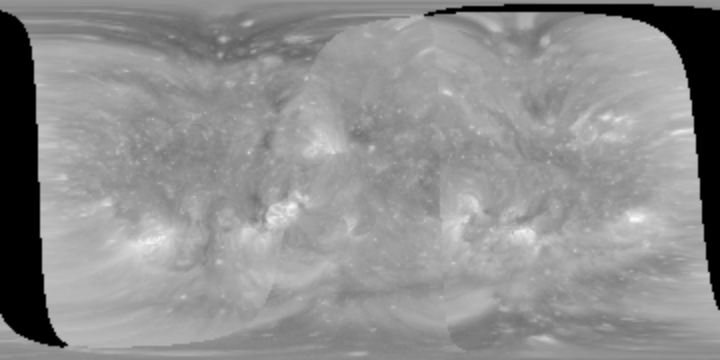
\includegraphics[width=0.47\linewidth]{pictures/segmentation_new_results/synoptic_GONG_20100807.png}
		\label{subfig:segmentation_EUVImage}}
	~\subfloat[Magnetic photomap image]{ 
		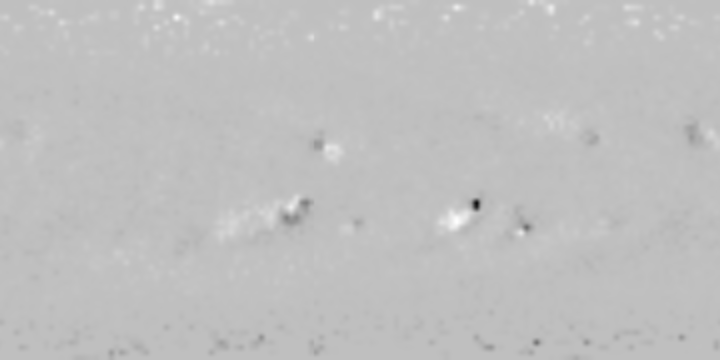
\includegraphics[width=0.47\linewidth]{pictures/segmentation_new_results/photomap_GONG_20100807.png}
		\label{subfig:segmentation_magnetic}} \\
	\subfloat[Consensus segmentaion]{ 
		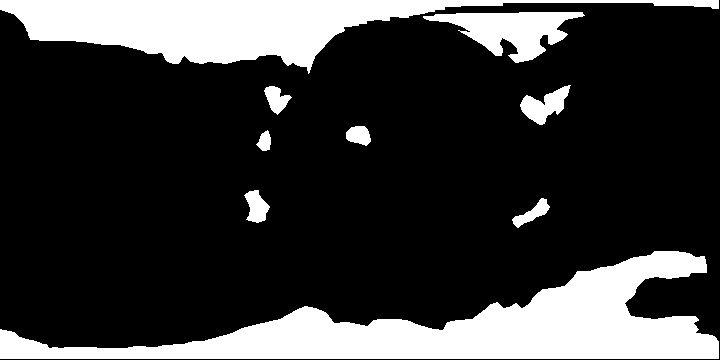
\includegraphics[width=0.47\linewidth]{pictures/segmentation_new_results/R8_1_drawn_euvi_new_20100807.png}
		\label{subfig:segmentation_consensus}
	}
	\subfloat[Henney-Harvey segmentation with Random Forest selection]{ 
		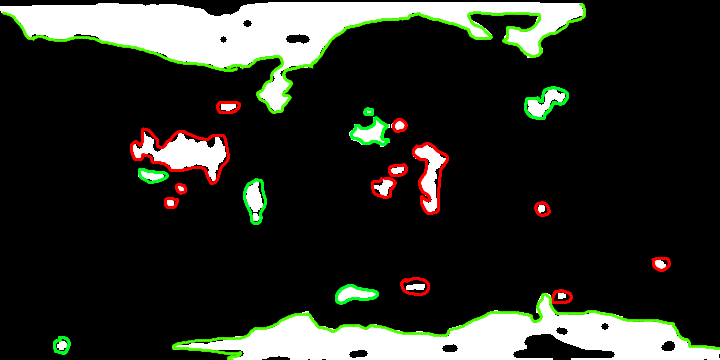
\includegraphics[width=0.47\linewidth]{pictures/segmentation_new_results/hh_20100807_painted.png}
		\label{subfig:segmentation_hh}
	}\\
	~\subfloat[FCN segmentation with \newline Random Forest selection]{ 
		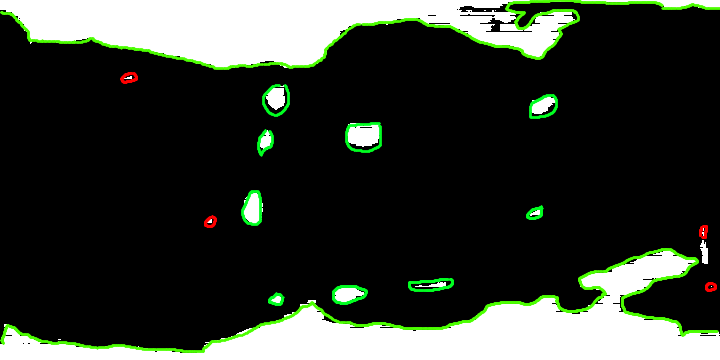
\includegraphics[width=0.47\linewidth]{pictures/segmentation_new_results/fcn_20100807_painted.png}
		\label{subfig:segmentation_fcn}
	}
	~\subfloat[SegNet segmentation with Random Forest selection]{ 
		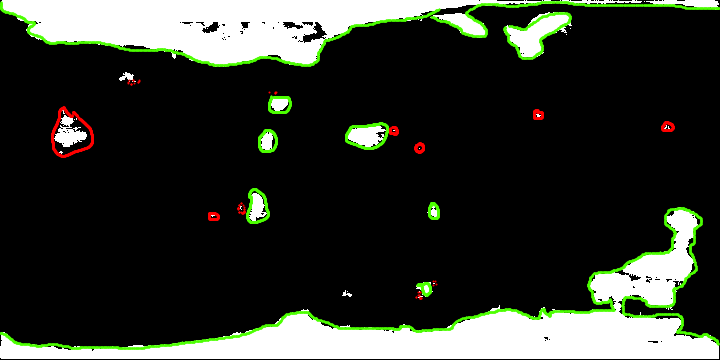
\includegraphics[width=0.47\linewidth]{pictures/segmentation_new_results/SegNets_20100807_painted.png}
		\label{subfig:segmentation_segnet}
	}\\
	~\subfloat[Level-sets segmentation \newline overlaid on EUV image]{ 
	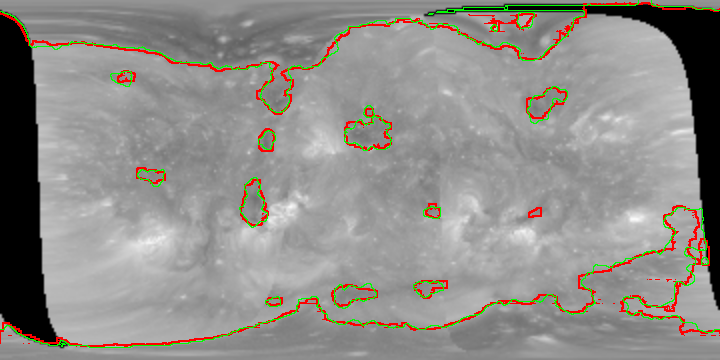
\includegraphics[width=0.47\linewidth]{pictures/segmentation_new_results/overlap_image.png}
	\label{subfig:ls}}
	~\subfloat[Proposed segmentation method vs Consensus map]{ 
		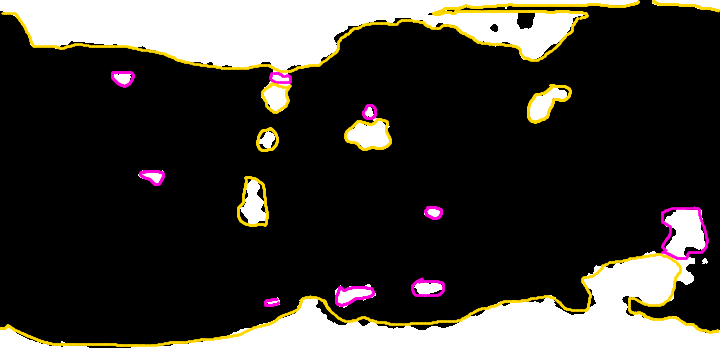
\includegraphics[width=0.47\linewidth]{pictures/segmentation_new_results/LS_on_FullCombo_20100807_painted.png}
		\label{subfig:gtls}
	}
	\caption{\label{fig:segmentation}
		\color{blue}
		Proposed segmentation method for the test date case of 8-7-2010.
	}        
\end{figure}
